\documentclass[11pt]{article}

\usepackage[margin=1.1in]{geometry}
\usepackage[utf8]{inputenc}
\usepackage[T1]{fontenc}
% θ appears inside \code{} spans in prose; listings' literate map only covers
% listings, so give inputenc a definition for the raw character.
\DeclareUnicodeCharacter{03B8}{\ensuremath{\theta}}
\usepackage{amsmath,amssymb}
\usepackage{booktabs}
\usepackage{listings}
\usepackage{xcolor}
\usepackage{tikz}
\usetikzlibrary{positioning,arrows.meta}
\usepackage{microtype}
\usepackage[hidelinks]{hyperref}

% Same plain Julia listing style as sampler_design.tex.
\lstdefinelanguage{Julia}{
  keywords={abstract,type,struct,mutable,function,end,if,else,elseif,for,
            while,begin,return,using,import,export,const,where,in,do,let,
            quote,macro,module,true,false,nothing,missing,local,global},
  sensitive=true,
  morecomment=[l]{\#},
  morestring=[b]",
}
\lstset{
  language=Julia,
  basicstyle=\ttfamily\small,
  keywordstyle=\bfseries,
  commentstyle=\color{black!55}\itshape,
  stringstyle=\color{black!70},
  showstringspaces=false,
  columns=fullflexible,
  keepspaces=true,
  breaklines=true,
  breakatwhitespace=true,
  frame=single,
  framerule=0.3pt,
  xleftmargin=1em,
  xrightmargin=1em,
  aboveskip=0.8\baselineskip,
  belowskip=0.8\baselineskip,
  literate={θ}{{$\theta$}}1
           {∂}{{$\partial$}}1
           {Σ}{{$\Sigma$}}1
           {≤}{{$\le$}}1
           {≥}{{$\ge$}}1
           {∈}{{$\in$}}1
           {∞}{{$\infty$}}1
           {·}{{$\cdot$}}1
           {—}{{---}}1
           {–}{{--}}1,
}

\newcommand{\E}{\mathbb{E}}
\newcommand{\dd}{\mathrm{d}}
\newcommand{\code}[1]{\texttt{#1}}

\title{Three Layers for a Queueing Library:\\
Surface Syntax, a GSMP Intermediate Representation,\\
and CompetingClocks}
\author{WorldTimer research notes}
\date{July 11, 2026}

\begin{document}
\maketitle
\tableofcontents

%==============================================================================
\section{What this document is}

This note makes the three-layer architecture for a queueing library concrete.
Layer~1 is the surface language a user types: stations, disciplines, routing.
Layer~2 is an intermediate representation (IR): a generalized semi-Markov
process (GSMP) written down as a plain data structure, together with a small
generic interpreter. Layer~3 is CompetingClocks.jl, which samples the clocks.
The document shows the surface syntax for five standard models, then compiles
one of them --- a size-based server farm --- down to the IR, rule by rule, and
shows exactly which CompetingClocks and ChronoSim calls the interpreter makes.

Four decisions, settled in discussion, are taken as given.

\begin{enumerate}
\item \textbf{Clock speeds are compiled away.} The GSMP literature gives each
  clock a state-dependent speed; CompetingClocks speaks distributions of firing
  times, including time-varying hazards. Section~\ref{sec:timechange} states
  the equivalence precisely: a speed is a deterministic time change of the
  clock's internal age, and every speed change compiles to a re-enabling with a
  left-truncated, rescaled distribution. The sampler never sees a speed.
\item \textbf{No one-input-queue rule.} Quarton's structural restriction
  (every server reads exactly one queue) made every model a state-machine
  Petri net and priced out fork--join and multiserver jobs. The IR allows
  synchronization; the surface language exposes it as \code{fork!}/\code{join!}.
\item \textbf{Record, then analyze.} Following ChronoSim, CompetingClocks, and
  ClockGradients, the primary observable is the trajectory record --- the
  ordered (clock key, firing time) sequence. Every queueing statistic is a fold
  over that record (Section~\ref{sec:measurement}). Accumulating state inside
  tokens or queues is not part of the design.
\item \textbf{Full-featured target.} The library should support time-varying
  hazards, static model checking, and derivative estimation through the
  ClockGradients contract. The IR is designed so that the checker and the
  estimators read the \emph{same} data structure the simulator runs.
\end{enumerate}

\begin{figure}[ht]
\centering
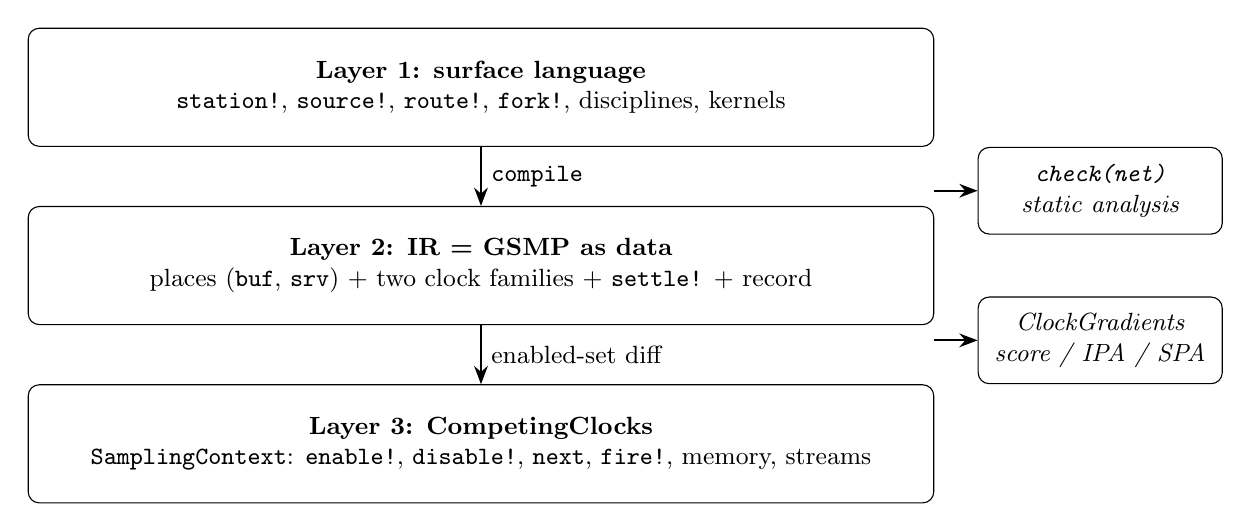
\begin{tikzpicture}[
  layer/.style={draw, rounded corners, minimum width=11.5cm, minimum height=1.5cm,
                align=center, font=\small},
  side/.style={draw, rounded corners, minimum width=3.1cm, minimum height=1.1cm,
               align=center, font=\small\itshape},
  arr/.style={-{Stealth}, thick},
]
\node[layer] (l1) {\textbf{Layer 1: surface language}\\
  \code{station!}, \code{source!}, \code{route!}, \code{fork!}, disciplines, kernels};
\node[layer, below=0.75cm of l1] (l2) {\textbf{Layer 2: IR = GSMP as data}\\
  places (\code{buf}, \code{srv}) + two clock families + \code{settle!} + record};
\node[layer, below=0.75cm of l2] (l3) {\textbf{Layer 3: CompetingClocks}\\
  \code{SamplingContext}: \code{enable!}, \code{disable!}, \code{next}, \code{fire!}, memory, streams};
\node[side, right=0.55cm of l2, yshift=0.95cm] (check) {\code{check(net)}\\static analysis};
\node[side, right=0.55cm of l2, yshift=-0.95cm] (grad) {ClockGradients\\score / IPA / SPA};
\draw[arr] (l1) -- node[right, font=\small]{\code{compile}} (l2);
\draw[arr] (l2) -- node[right, font=\small]{enabled-set diff} (l3);
\draw[arr] (l2.east|-check.west) -- (check.west);
\draw[arr] (l2.east|-grad.west) -- (grad.west);
\end{tikzpicture}
\caption{The three layers. The checker and the derivative estimators attach to
the IR, not to the surface language and not to the sampler.}
\label{fig:layers}
\end{figure}

The one-sentence contract of each layer:

\begin{itemize}
\item \emph{Layer 1 builds a value.} The surface calls construct a
  \code{QueueNetwork}; nothing executes.
\item \emph{Layer 2 is five pure functions over data.} Compilation produces a
  \code{QueueGSMP} that satisfies exactly the ClockGradients model contract:
  \code{initial\_state}, \code{clockkeytype}, \code{enabled},
  \code{clock\_distribution}, \code{fire}.
\item \emph{Layer 3 is driven by diffs.} No rule ever calls the sampler.
  The interpreter compares \code{enabled(state)} before and after a firing and
  issues \code{enable!}/\code{disable!} for the difference --- the same pattern
  as ClockGradients' \code{ClockWorld} and ChronoSim's reactive engine.
\end{itemize}

%==============================================================================
\section{Layer 1: the surface language}

\subsection{Vocabulary}

The surface language has six term constructors. Each builds an entry in a
\code{QueueNetwork} value; none has side effects beyond that.

\begin{center}
\small
\begin{tabular}{@{}lll@{}}
\toprule
Constructor & Arguments & Meaning \\
\midrule
\code{source!} & interarrival law, mark sampler & jobs enter here \\
\code{station!} & discipline, servers, service law, capacity & jobs are served here \\
\code{sink!} & --- & jobs leave here \\
\code{fork!} & branch list & one job becomes siblings \\
\code{join!} & part count & siblings merge when all arrive \\
\code{route!} & origin, routing kernel & where departures go \\
\bottomrule
\end{tabular}
\end{center}

A \emph{law} is always a function of \code{(θ, t)} or \code{(job, θ, t)}
returning a \code{Distributions.UnivariateDistribution}: \code{θ} is the global
parameter vector (the seam every derivative estimator differentiates through),
and \code{t} is the wall-clock enabling time, which is what makes time-varying
hazards --- a nonhomogeneous arrival process, a repair rate with a shift
schedule --- expressible with no extra machinery. A \emph{mark} is a named
value attached to a job at creation (its size, its class); marks are what
disciplines and routing kernels read.

\subsection{A discipline is four functions}
\label{sec:discipline}

The design finding that reorganizes Quarton: a service discipline is not a
queue subtype. It is a value with four small pure functions, and the buffer is
always the same ordered vector.

\begin{lstlisting}
struct Discipline
    insert    # (buf, jobid, state) -> position at which the job is filed
    select    # (buf, state) -> jobid to admit to a free server, or nothing
    preempt   # (state, station) -> jobid in service to evict, or nothing
    memory    # :fresh | :resume | :replay  (what an evicted clock remembers)
end
\end{lstlisting}

The \code{memory} field is the generalized-stochastic-Petri-net (GSPN)
preemption vocabulary, and it maps directly onto ChronoSim's per-event
\code{memory\_policy} declaration: \code{:fresh} is preemptive-repeat-different
(a re-enabled clock starts over), \code{:resume} banks the enabled age across
the disable (ChronoSim implements this by left-shifting the enabling time it
hands the sampler), and \code{:replay} repeats the identical draw
(CompetingClocks' \code{supports\_retained\_draw} backends). Standard
disciplines are instances:

\begin{center}
\small
\begin{tabular}{@{}lllll@{}}
\toprule
Discipline & \code{insert} & \code{select} & \code{preempt} & \code{memory} \\
\midrule
\code{FCFS()}            & back           & front   & never & --- \\
\code{LCFS(:resume)}     & front          & front   & arriving job evicts & \code{:resume} \\
\code{SIRO()}            & back           & uniform draw & never & --- \\
\code{Priority(by)}      & ordered by key & front   & never & --- \\
\code{Priority(by, preempt=true)} & ordered by key & front & lower key in service & \code{:resume} \\
\code{SRPT()}            & by remaining size & front & larger remainder in service & \code{:resume} \\
\code{ProcessorSharing()} & \multicolumn{4}{l}{no buffer: every job is in service; see Section~\ref{sec:timechange}} \\
\bottomrule
\end{tabular}
\end{center}

Two disciplines need a word. \code{SRPT} requires the remaining size of a job
in service, which is its size mark minus the clock's enabled age; the IR can
read ages because CompetingClocks exposes \code{enabled\_ages} (any
\code{supports\_enabled\_ages} backend). \code{SIRO}'s uniform draw is
randomness outside any clock; Section~\ref{sec:randomness} accounts for it.

\subsection{Routing kernels}

Both of Quarton's mechanisms --- the server's disbursement policy and the
queue's hard-coded dispatch --- collapse into one concept. A routing kernel is
a function \code{(job, state) -> station id} attached to the \emph{origin}
station. State-dependent kernels read buffer lengths or work backlogs from the
state; stateful kernels (round robin) declare their cursor, and the cursor
lives in the IR state so that record replay reproduces it.

\begin{lstlisting}
Always(dest)                      # every departure goes to dest
Probabilistic(dest1 => p1, ...)   # Markovian routing (a random draw)
ByMark(f)                         # f(job) names the destination: SITA
JoinShortestQueue(dests)          # reads buffer lengths from state
LeastWorkLeft(dests)              # reads remaining-work backlogs from state
RoundRobin(dests)                 # stateful: cursor is IR state
\end{lstlisting}

\subsection{Five models in the syntax}

\textbf{M/M/1.} The smallest complete program.

\begin{lstlisting}
net = QueueNetwork(param_names = (:lambda, :mu))
source!(net, :arrive; interarrival = (θ, t) -> Exponential(inv(θ[1])))
station!(net, :counter; discipline = FCFS(), servers = 1,
         service = (job, θ, t) -> Exponential(inv(θ[2])))
sink!(net, :done)
route!(net, :arrive, Always(:counter))
route!(net, :counter, Always(:done))
\end{lstlisting}

\textbf{SITA farm (size-interval task assignment).} Jobs carry a size mark;
routing reads it; each service law scales by it. This is the example compiled
end-to-end in Section~\ref{sec:worked}.

\begin{lstlisting}
net = QueueNetwork(param_names = (:lambda, :mu_short, :mu_long))
source!(net, :arrive;
        interarrival = (θ, t) -> Exponential(inv(θ[1])),
        mark = rng -> (size = rand(rng, LogNormal(0.0, 1.0)),))
station!(net, :short; discipline = FCFS(), servers = 1,
         service = (job, θ, t) -> Exponential(job.size * inv(θ[2])))
station!(net, :long;  discipline = FCFS(), servers = 1,
         service = (job, θ, t) -> Exponential(job.size * inv(θ[3])))
sink!(net, :done)
route!(net, :arrive, ByMark(job -> job.size < 2.0 ? :short : :long))
route!(net, :short, Always(:done)); route!(net, :long, Always(:done))
\end{lstlisting}

\textbf{Preemptive priority, M/G/1.} The discipline carries the preemption
rule and the memory policy; the service law is Weibull, so \code{:resume}
is observably different from \code{:fresh}.

\begin{lstlisting}
station!(net, :cpu;
    discipline = Priority(job -> job.class; preempt = true, memory = :resume),
    servers = 1,
    service = (job, θ, t) -> Weibull(θ[2], θ[3]))
\end{lstlisting}

\textbf{M/M/1--PS (processor sharing).} Only the discipline changes; the
compiler does the work (Section~\ref{sec:timechange}).

\begin{lstlisting}
station!(net, :cpu; discipline = ProcessorSharing(), servers = 1,
         service = (job, θ, t) -> Exponential(inv(θ[2])))
\end{lstlisting}

\textbf{Fork--join.} Legal now that the one-input rule is gone. A job splits
into two siblings that queue at separate disk stations; the join holds each
sibling until its partner arrives.

\begin{lstlisting}
fork!(net, :split; branches = (:disk_a, :disk_b))
station!(net, :disk_a; discipline = FCFS(), servers = 1,
         service = (job, θ, t) -> Gamma(2.0, inv(θ[2])))
station!(net, :disk_b; discipline = FCFS(), servers = 1,
         service = (job, θ, t) -> Gamma(2.0, inv(θ[3])))
join!(net, :merge; parts = 2)
route!(net, :disk_a, Always(:merge)); route!(net, :disk_b, Always(:merge))
route!(net, :merge, Always(:done))
\end{lstlisting}

A closed network needs no new constructs: route the last station back to the
first and start \code{initial\_jobs} at chosen stations instead of declaring a
source.

%==============================================================================
\section{Layer 2: the intermediate representation}

\subsection{The data structure}

Compilation (\code{compile(net) -> QueueGSMP}) turns the surface value into
pure data plus per-station function fields. Nothing here is a framework: it is
a struct you can print, diff, hash, and analyze.

\begin{lstlisting}
struct CompiledStation
    kind::Symbol          # :source | :station | :sink | :fork | :join
    servers::Int
    capacity::Int         # typemax(Int) when unbounded
    overflow::Symbol      # :drop | :block
    discipline::Discipline
    service::Function     # (job, θ, t) -> UnivariateDistribution
    routing::Function     # (job, state) -> station index
    mark::Function        # sources only: rng -> NamedTuple
    parts::Int            # joins only: siblings to await
end

struct QueueGSMP
    stations::Vector{CompiledStation}
    names::Dict{Symbol,Int}
end
\end{lstlisting}

The dynamic state is places. The buffer order \emph{is} the discipline's
data --- Shedler's job stack --- so there is no per-discipline container type.

\begin{lstlisting}
struct QueueState
    buf::Vector{Vector{JobId}}     # per station, in discipline order
    srv::Vector{Vector{JobId}}     # per station, the jobs in service
    jobs::Dict{JobId,Job}          # class, marks, birth time index
    pending::Vector{Dict{GroupId,Vector{JobId}}}  # joins: siblings so far
    cursor::Vector{Int}            # stateful routing kernels live in state
    next_id::JobId                 # deterministic job identity for replay
end
\end{lstlisting}

There are exactly two clock families, so the clock key type is one concrete
isbits tuple, the way ChronoSim's \code{clock\_key} flattens an event struct:

\begin{lstlisting}
const ClockKey = Tuple{Symbol,Int32,Int64}
# (:arrival, station, 0)      the source's next-arrival clock
# (:service, station, jobid)  one clock per job in service
\end{lstlisting}

The enabled-set function is a fixed loop over the state --- deterministic
order, as the ClockGradients contract requires:

\begin{lstlisting}
function enabled(m::QueueGSMP, st::QueueState)
    ks = ClockKey[]
    for s in eachindex(m.stations)
        m.stations[s].kind == :source && push!(ks, (:arrival, Int32(s), 0))
        for j in st.srv[s]
            push!(ks, (:service, Int32(s), j))
        end
    end
    return ks
end
\end{lstlisting}

\subsection{Station-to-rule compilation}
\label{sec:compilation}

The entire dynamic semantics is one \code{fire} function, one \code{deposit!}
helper, and one normalization function \code{settle!}. Everything a station
means at run time is which branches of these three functions its fields select.
No rule touches the sampler; \code{fire} is a pure state-to-state map
(ClockGradients' contract), and clock lifecycle is implied by the change in
\code{enabled(state)}.

\begin{lstlisting}
function fire(m::QueueGSMP, st::QueueState, key::ClockKey)
    st = fresh_copy(st)                    # fire is pure: never mutate input
    fam, s, j = key
    if fam == :arrival
        job = create_job!(st, m, s)        # draws marks; Section 3.5
        deposit!(m, st, m.stations[s].routing(job, st), job.id)
    else
        delete_from_service!(st, s, j)     # the (:service,s,j) clock vanishes
        deposit!(m, st, m.stations[s].routing(st.jobs[j], st), j)
        settle!(m, st, s)                  # the freed slot may admit a job
    end
    return st
end
\end{lstlisting}

\begin{lstlisting}
function deposit!(m::QueueGSMP, st::QueueState, d::Int, j::JobId)
    stn = m.stations[d]
    if stn.kind == :sink
        remove_job!(st, j)                 # departure is visible in the record
    elseif stn.kind == :fork
        for b in stn.branches              # siblings share a group id
            deposit!(m, st, b, sibling!(st, j, b))
        end
    elseif stn.kind == :join
        stash_sibling!(st, d, j)
        if all_parts_present(st, d, j)
            file_into_buffer!(st, d, merge_siblings!(st, d, j))
            settle!(m, st, d)
        end
    else                                   # an ordinary station
        if buffer_full(st, stn, d)
            stn.overflow == :drop ? remove_job!(st, j) : block!(st, d, j)
        else
            file_into_buffer!(st, d, j)    # position := discipline.insert
            settle!(m, st, d)
        end
    end
end
\end{lstlisting}

\begin{lstlisting}
function settle!(m::QueueGSMP, st::QueueState, q::Int)
    disc = m.stations[q].discipline
    # 1. Preemption: may the best waiting job evict a job in service?
    while (evict = disc.preempt(st, q)) !== nothing
        move_to_buffer!(st, q, evict)      # its clock leaves the enabled set;
    end                                    # disc.memory says what its next
                                           # enabling means (age or no age)
    # 2. Dispatch: fill free slots in discipline order.
    while length(st.srv[q]) < m.stations[q].servers
        j = disc.select(st.buf[q], st)
        j === nothing && break
        move_to_service!(st, q, j)         # its clock joins the enabled set
    end
end
\end{lstlisting}

That is the whole compilation scheme. The correspondence, feature by feature:

\begin{center}
\small
\begin{tabular}{@{}ll@{}}
\toprule
Surface feature & Where it lands in the IR \\
\midrule
source interarrival law & distribution of the \code{(:arrival, s, 0)} clock \\
service law & distribution of \code{(:service, s, j)} clocks \\
discipline \code{insert}/\code{select} & \code{file\_into\_buffer!} position; \code{settle!} step 2 \\
discipline \code{preempt}/\code{memory} & \code{settle!} step 1; clock memory on re-enable \\
routing kernel & the destination argument of \code{deposit!} \\
finite capacity, \code{:drop}/\code{:block} & the \code{buffer\_full} branch of \code{deposit!} \\
fork, join & the \code{:fork}/\code{:join} branches of \code{deposit!} \\
sink & job removal; the departure survives in the record \\
\bottomrule
\end{tabular}
\end{center}

The sub-event ordering worry from Quarton's \code{definition.md} --- ``the
danger of separating these steps is that we might exclude a useful model'' ---
is resolved by fiat here: within one firing, the cascade order is
\code{deposit!} at the destination, then \code{settle!} at the destination,
then \code{settle!} at the origin. The order is part of the IR's semantics, it
is deterministic, and because \code{fire} is pure it is the \emph{same} order
the record fold replays.

\subsection{Worked compilation: the SITA farm}
\label{sec:worked}

The Layer-1 program in Section 2.4 compiles to:

\begin{itemize}
\item \emph{Places.} \code{buf} and \code{srv} vectors indexed by
  \{1 \code{arrive}, 2 \code{short}, 3 \code{long}, 4 \code{done}\}; only
  stations 2 and 3 use theirs.
\item \emph{Clocks.} \code{(:arrival, 1, 0)} always enabled;
  \code{(:service, 2, j)} for the job \code{j} occupying \code{short}'s
  server; \code{(:service, 3, j)} likewise for \code{long}.
\item \emph{Laws.} \code{clock\_distribution} dispatches on the key's family:
\begin{lstlisting}
function clock_distribution(m::QueueGSMP, θ, key, st)
    fam, s, j = key
    stn = m.stations[s]
    fam == :arrival && return stn.service(nothing, θ, st.time)
    return stn.service(st.jobs[j], θ, st.time)   # reads job.size
end
\end{lstlisting}
\end{itemize}

One arrival, traced through the interpreter, with the state
``\code{short}'s server busy with job 7, buffers empty'':

\begin{enumerate}
\item The sampler reports \code{(:arrival, 1, 0)} fires at $t^\ast$.
\item \code{fire} runs: \code{create\_job!} makes job 9, draws its mark
  (\code{size} $= 1.3$), and \code{ByMark} routes it to station 2
  (\code{short}) because $1.3 < 2.0$.
\item \code{deposit!} files job 9 at the back of \code{buf[2]} (FCFS
  \code{insert}); \code{settle!(2)} finds no free slot (job 7 holds it) and
  no preemption (FCFS never preempts). Job 9 waits.
\item The interpreter diffs the enabled sets: before
  $= \{(\text{:arrival},1,0), (\text{:service},2,7)\}$, after adds nothing
  and removes only the fired arrival clock, which is immediately re-enabled
  fresh --- one \code{enable!} call with
  \code{Exponential(inv(θ[1]))} at $t^\ast$.
\item Later \code{(:service, 2, 7)} fires: job 7 departs to \code{done}
  (removed), \code{settle!(2)} admits job 9, and the diff enables
  \code{(:service, 2, 9)} with \code{Exponential(1.3 * inv(θ[2]))}.
\end{enumerate}

Every number in that trace is reconstructible from the record
$((\text{:arrival},1,0), t^\ast), ((\text{:service},2,7), t'), \ldots$ by
folding \code{fire} --- which is what makes the measurement layer and the
estimators work on the record alone.

\subsection{Preemption, processor sharing, and the time-change proposition}
\label{sec:timechange}

\textbf{Terminology accord.} Let a clock be enabled at wall time $t_e$ with
service requirement $X \sim F$ (hazard $h_F$), and let it run at a
state-dependent speed $r(t) \ge 0$ that is constant between events of the
process. Define the internal age $a(t) = \int_{t_e}^{t} r(u)\,\dd u$. The
clock fires at
\[
T \;=\; \inf\{\, t : a(t) \ge X \,\},
\]
and between events its wall-clock hazard is $r(t)\, h_F(a(t))$. So ``a GSMP
with clock speeds'' and ``a GSMP whose clocks carry (possibly time-varying)
firing-time distributions, updated at event boundaries'' are the same object:
the speed is a deterministic time change of the age. Operationally, when an
event changes the speed from $r_1$ to $r_2$ at time $t_1$ with banked internal
age $a_1$, the clock's remaining wall-clock lifetime is
\[
\frac{(X - a_1)}{r_2} \;\Bigm|\; X > a_1
\qquad\text{i.e.}\qquad
\code{scale(LeftTruncated(F, a1) - a1, 1/r2)},
\]
a left-truncation and rescale of $F$ --- both operations CompetingClocks
already owns (\code{distributions/lefttrunc.jl}; scaling is
Distributions.jl). One care point: this compiled re-enabling is anchored at
the \emph{current} time because the age bookkeeping has moved into the
truncation; returning the original enabling time as well (the usual
\code{reenable} idiom for keeping age) would count the age twice.

\textbf{Preemption} uses the same machinery at speed zero: an evicted job's
clock leaves the enabled set; under \code{memory = :resume} its banked age
$a_1$ is applied as the truncation point when it re-enters service
(ChronoSim's \code{:resume} policy does exactly this by shifting the enabling
time); under \code{:fresh} the bank is discarded.

\textbf{Processor sharing} compiles to: all $n$ jobs at the station sit in
\code{srv}, each with speed $k/n$ ($k$ servers shared by $n$ jobs). Every
arrival to or departure from the station changes $n$, so the interpreter
re-enables each resident clock with its truncated, rescaled remainder. Two
execution paths support this: ChronoSim's \code{reenable} seam re-evaluates
in-flight clocks natively, and the ClockGradients four-argument
\code{clock\_distribution(model, θ, key, state)} form exists for exactly this
mid-flight re-evaluation. The pure \code{ClockWorld} runner freezes
distributions at enabling and is therefore \emph{not} sufficient for PS; the
capability table in Section~\ref{sec:estimators} records this honestly.

\subsection{Randomness accounting: marks and routing draws}
\label{sec:randomness}

A GSMP puts all randomness in clocks. Queueing adds two draws that are not
clocks, and the design must say where they live because the likelihood --- and
therefore the score estimator --- depends on it.

\begin{itemize}
\item \emph{Job marks} (the size drawn at arrival). The draw happens inside
  \code{fire} of the arrival clock. ChronoSim's \code{CountingRNG} already
  flags fire-randomness; here we make it lawful instead of merely flagged. If
  the mark density $g_\theta$ is $\theta$-free (the SITA example: a fixed
  LogNormal), the likelihood factor is constant and the score is untouched.
  If marks depend on $\theta$, the trajectory log-likelihood gains a term per
  arrival:
  \[
  \log L(\theta) \;=\;
  \underbrace{\sum_i \Big[ \log h_{k_i}(t_i)
    - \sum_{j \in E(t_{i-1},t_i]} \int h_j \Big]}_{\text{clock part: ChronoSim's \code{trace\_likelihood}}}
  \;+\;
  \underbrace{\sum_{\text{arrivals } a} \log g_\theta(\text{mark}_a)}_{\text{mark part: new}} .
  \]
  The record must therefore store marks alongside arrival firings (a
  \emph{marked} record), which is also what the measurement layer wants.
\item \emph{Routing draws} (\code{Probabilistic}, \code{SIRO}'s pick). Same
  treatment: a discrete density factor, $\theta$-free unless the user
  parameterizes routing probabilities by $\theta$, in which case the factor
  $\log p_\theta(\text{choice})$ joins the likelihood. Deterministic kernels
  (\code{ByMark}, \code{JSQ}, \code{LWL}, \code{RoundRobin} with its cursor in
  state) contribute nothing and keep \code{fire} a deterministic function of
  \code{(state, key, marks)} --- the property the record fold and the pathwise
  estimators prefer.
\end{itemize}

This gives a crisp rule the checker can enforce: \emph{every random draw in
the system is either a clock, a recorded mark with a density, or a recorded
choice with a probability mass.} Nothing else may touch an RNG.

\subsection{The record and the measurement layer}
\label{sec:measurement}

The primary output of a run is the marked record
\[
\mathcal{R} = \big( (k_1, t_1, m_1), (k_2, t_2, m_2), \ldots \big),
\qquad k_i \in \text{ClockKey},\; m_i = \text{marks if } k_i \text{ is an arrival},
\]
plus the horizon --- ChronoSim's \code{MinimalRecord} with the mark column
added. Because \code{fire} is pure and deterministic given marks, the state at
any index is a fold, and the OB-1 measurements showed the fold is
\emph{cheaper} than re-running the engine. Every statistic in
Harchol-Balter's book is a fold over $\mathcal{R}$:

\begin{lstlisting}
lifecycle = job_events(m, rec)
# folds fire over rec once, emitting per-job daters:
#   (jobid, :created,     station, t)
#   (jobid, :entered_buf, station, t)
#   (jobid, :entered_srv, station, t)   # also re-entries after preemption
#   (jobid, :departed,    station, t)

response(lifecycle)     # departed - created, per job
wait(lifecycle, :short) # entered_srv - entered_buf at one station
number_in_system(rec)   # a counting-process integral, exact between events
utilization(rec, :short)
\end{lstlisting}

Shedler's passage-time queries become a two-predicate fold, which is his
marked-job specification with the record replacing the state augmentation ---
the record already contains what his 1987 memory budget forced him to
compress:

\begin{lstlisting}
passage_times(lifecycle;
    enter = ev -> ev.kind == :entered_buf && ev.station == :split,
    exit  = ev -> ev.kind == :departed    && ev.station == :merge)
\end{lstlisting}

Streaming observers remain possible (fold incrementally during the run instead
of after it) for long runs where storing $\mathcal{R}$ hurts, but they are an
execution-policy choice, not a modeling concept --- the same fold, run early.

\subsection{Model checking on the IR}
\label{sec:checking}

Because the IR is data, checks are total functions of it, not lint heuristics
over user callbacks. \code{check(net)} runs at compile time:

\begin{itemize}
\item[C1.] \emph{Structure.} Every routing target exists; every station
  reaches a sink (or the network is declared closed); every fork's branches
  reach a common join or sinks; every join's \code{parts} matches its fork.
\item[C2.] \emph{Mark typing.} \code{ByMark}/\code{SRPT}/\code{Priority}
  require the marks they read to be produced by every source whose jobs can
  reach them --- a dataflow check over the routing graph.
\item[C3.] \emph{Capacity.} Finite buffers declare \code{:drop} or
  \code{:block}; blocking chains must be acyclic (a cycle of full blocking
  buffers is deadlock, detected statically).
\item[C4.] \emph{Stability.} Solve the traffic equations for visit ratios,
  estimate $\rho_s = \lambda_s \E[S_s]/k_s$ where the laws permit a mean at
  the given $\theta$, and warn when $\rho_s \ge 1$.
\item[C5.] \emph{Oracle detection.} If every station satisfies the BCMP
  conditions (FCFS with exponential class-independent service, or PS, or
  LCFS-preempt-resume, or infinite-server) and routing is state-independent,
  emit the product-form stationary distribution as a test oracle. Small
  all-exponential networks additionally get an exact CTMC oracle by state
  enumeration. This is how the repo's 4-standard-error test convention gets
  its exact answers for free.
\item[C6.] \emph{Randomness census.} List every mark and routing draw with its
  $\theta$-dependence, and report which estimators are valid
  (the tier table in Section~\ref{sec:estimators}).
\end{itemize}

Runtime invariants (debug builds, ChronoSim's invariant machinery): job
conservation off-source/off-sink; \code{buf} and \code{srv} disjoint;
\code{enabled(state)} agreeing with the sampler's enabled set after every
firing.

%==============================================================================
\section{Layer 3: CompetingClocks, and the two integrations}

\subsection{The sampler mapping}

The interpreter drives the blessed \code{SamplingContext} surface. The
complete mapping:

\begin{center}
\small
\begin{tabular}{@{}ll@{}}
\toprule
IR notion & CompetingClocks realization \\
\midrule
clock key & the \code{ClockKey} tuple; context built with this key type \\
clock born (diff: appears)     & \code{enable!(ctx, key, dist, te, now)} \\
clock cancelled (diff: leaves) & \code{disable!(ctx, key, now)} \\
winner \& time  & \code{next(ctx, now)}; then \code{fire!(ctx, key, t)} \\
\code{:resume} memory & enabling-time shift; \code{supports\_enabled\_ages} backends \\
\code{:replay} memory & \code{supports\_retained\_draw} backends \\
speed change / PS & re-enable with \code{LeftTruncated} + rescale (Sec.~\ref{sec:timechange}) \\
time-varying hazard & any \code{UnivariateDistribution}; \code{hazard(d, te, t)} is generic \\
SRPT's remaining size & \code{enabled\_ages(ctx, now)} \\
record & \code{TrajectoryRecorder} / ChronoSim \code{MinimalRecord} \\
reproducibility & keyed streams from one master seed (\code{KeyedStreams}) \\
sampler choice & \code{SamplerBuilder}: \code{NextReactionMethod} default; \\
& \code{FirstToFireMethod(coupling=:carry)} when IPA wants the carry coupling \\
\bottomrule
\end{tabular}
\end{center}

Non-exponential laws are first-class throughout --- that is the reason
CompetingClocks exists --- so ``time-varying hazards for rates'' costs the
surface language nothing: the law functions already receive \code{t}.

\subsection{Embedding in ChronoSim: two event families}

The IR needs no code generation to run under ChronoSim. Two generic
\code{SimEvent} structs cover every network, because all model specificity
lives in the \code{QueueGSMP} value carried by the physical state:

\begin{lstlisting}
struct Arrival <: SimEvent
    station::Int32
end
struct Service <: SimEvent
    station::Int32
    job::Int64
end

precondition(e::Arrival, phys) = true    # a source is always live
precondition(e::Service, phys) = e.job in phys.state.srv[e.station]

enable(e::Arrival, phys, θ, when) =
    (phys.net.stations[e.station].service(nothing, θ, when), when)
enable(e::Service, phys, θ, when) =
    (phys.net.stations[e.station].service(phys.state.jobs[e.job], θ, when), when)

fire!(e::Service, phys, when, rng) =
    apply!(phys, fire(phys.net, phys.state, (:service, e.station, e.job)))

memory_policy(::Type{Service}) = :resume   # per-network, from the disciplines
\end{lstlisting}

ChronoSim's generators watch the \code{srv} places and propose \code{Service}
events when jobs enter service; its \code{reenable} seam implements the PS
rescaling; its \code{RecordMinimal} policy captures the record. The dynamic
semantics of the whole queueing library is those two event families plus
\code{settle!} --- everything else is data.

\subsection{Satisfying the ClockGradients contract}
\label{sec:estimators}

\code{QueueGSMP} implements the five-function model contract directly ---
\code{initial\_state}, \code{clockkeytype}, \code{enabled},
\code{clock\_distribution} (the four-argument, state-dependent form), and
\code{fire} --- with one honest wrinkle: the contract's \code{fire} is pure
and deterministic, and arrivals draw marks. The resolution is the marked
record: during estimation, \code{fire} is evaluated \emph{given} the recorded
marks, which restores determinism exactly the way the likelihood conditions on
them. The estimator files then apply unchanged; what varies by network feature
is which estimators are valid, and the checker's C6 census reports it:

\begin{center}
\small
\begin{tabular}{@{}lcccc@{}}
\toprule
Network feature & simulate & likelihood/score & IPA (carry) & SPA/branching \\
\midrule
exponential + FCFS, det.\ routing & \checkmark & \checkmark & \checkmark & \checkmark \\
general laws, time-varying hazards & \checkmark & \checkmark & \checkmark & \checkmark \\
$\theta$-free marks (SITA) & \checkmark & \checkmark & \checkmark & \checkmark \\
$\theta$-dependent marks & \checkmark & + mark term & mark pathwise$^{\ast}$ & open \\
$\theta$-dependent \code{Probabilistic} routing & \checkmark & + mass term & discrete: no & \checkmark \\
preempt-\code{:resume} & \checkmark & \checkmark & \checkmark & \checkmark \\
processor sharing (re-evaluation) & \checkmark & \checkmark & needs framework world & needs framework world \\
\bottomrule
\end{tabular}

{\footnotesize $^{\ast}$differentiable if the mark is a smooth transform of a
$\theta$-free draw --- the usual reparameterization condition.}
\end{center}

``Needs framework world'' marks the \code{ClockWorld} freeze-at-enabling
limitation: PS re-evaluates clocks mid-flight, so the branching estimators
must run over the ChronoSim-backed world, which re-enables through the
\code{reenable} seam.

The payoff, in the shape the repo's tests want: for the SITA farm,
\begin{lstlisting}
rec = simulate(net, θ; horizon = 200.0, seed = 90210)
W(θ) = mean(wait(job_events(compile(net), rec), :short))
# score: ForwardDiff over trace_likelihood + mark terms, weighted by W
# IPA:   carry-coupled replay of the record through clock_distribution
paired_estimate(net, θ, W; estimators = (:score, :ipa))
\end{lstlisting}
with C5's product-form oracle (this farm is two independent M/G/1 queues once
the size split is fixed, so the oracle is closed-form) providing the value
\emph{and} the derivative to test against.

%==============================================================================
\section{Design findings and open questions}

Findings this layering forces, stated as claims a prototype can test:

\begin{enumerate}
\item \emph{Two clock families suffice.} Arrival and Service cover sources,
  stations, forks, joins, and sinks; disciplines and routing never create new
  clock kinds, only new state-reading functions. If a queueing feature
  demands a third family, that is a discovery worth its own note.
\item \emph{A discipline is (insert, select, preempt, memory).} Quarton's
  queue subtypes and Assignment objects both dissolve into these four
  functions plus routing kernels.
\item \emph{Speeds compile to truncate-and-rescale re-enablings.} The sampler
  needs left-truncation, age reads, and per-clock memory --- all of which
  CompetingClocks has --- and nothing else.
\item \emph{The marked record is the single trajectory representation} for
  statistics, likelihoods, and derivatives; the mark column is the one
  extension queueing forces on \code{MinimalRecord}.
\item \emph{Checking is total because the model is a value.} The BCMP/CTMC
  oracle detector (C5) turns the checker into a test-oracle generator, which
  is the cheapest route to the repo's 4-standard-error test convention.
\end{enumerate}

Open questions, in rough order of how much they threaten the design:

\begin{enumerate}
\item \emph{Blocking cascades.} \code{:block} with transfer blocking can
  propagate a single departure through several full buffers. The
  \code{deposit!}/\code{settle!} order handles one hop; a chain needs a
  worklist, and the determinism argument must be redone for it.
\item \emph{SRPT's replay.} Preemption decisions read clock ages; the record
  fold can reconstruct ages from enabling times, but the IPA replay must
  differentiate through the preemption \emph{boundary} --- exactly the kind of
  discrete-decision discontinuity SPA exists for. Which estimator owns SRPT
  is unresolved.
\item \emph{$\theta$-dependent marks under SPA.} The branching estimators
  branch on clock order; a mark that shifts a routing decision is a second
  discontinuity source not covered by the current branchable-world verbs.
\item \emph{Stateful kernels in records.} \code{RoundRobin}'s cursor is IR
  state, so replay works; but a user-written stateful kernel that hides state
  in a closure breaks the fold silently. The surface API should make kernel
  state declarative (a field, not a closure), and the checker should reject
  closures it cannot see into.
\end{enumerate}

The next concrete step this note implies: a green-field \code{src/QueueLayers}
prototype that implements \code{QueueNetwork}, \code{compile},
\code{fire}/\code{deposit!}/\code{settle!}, the record fold, and checks
C1--C4, tested on M/M/1 and the SITA farm against C5-style closed-form
oracles --- with PS and preemption deferred to a second pass that exercises the
\code{reenable} path.

\end{document}
